\section{Chapter 4: Color}
\graphicspath{ {pngs/ch4/} }


\secttoc

Although color is the most studied feature of perception, the results are few.
Most important is opponent process theory.
This discussion continues in other chapters.

\begin{mdframed}\begin{multicols}{2}
\subsection{Trichromacy theory}
Color vision helped break camouflage. Color is more of an attribute than a
primary characteristic.
Chickens have 12 kinds of color-sensitive cells.
\begin{compactdesc}
    \item[Color] excellent for labeling or categorization. We have 3 kinds
        of color-sensitive cells. These three  colors can be mixed together
        to simulate other colors.
    \item[Cones]
        Rods are overstimulated at most light levels and rendered useless.
    \item[Color blindness] 10\% male, 1\% female. Most common is the lack of
        long-wavelength (protanopia) or medium-wavelength (deuternopia).
        Respectively, can't see red or green. 3D space collapses to 2D space.
\end{compactdesc}
    \begin{figure}[H]
        \centering
        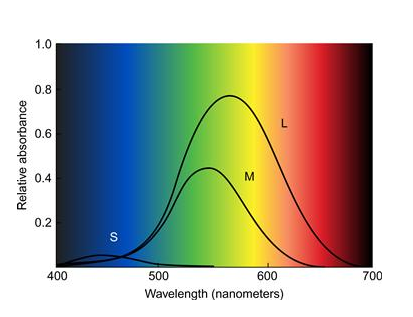
\includegraphics[width=0.4\textwidth]{cone_sensitivity.png}
        \caption{Cone sensitivity functions}
    \end{figure}


\end{multicols}\end{mdframed}


\begin{mdframed}\begin{multicols}{2}
\subsection{Color measurement}
\begin{compactdesc}
    \item[CIE tristimulus system] is the most precise, closest to our perceptive
        abilities.
    \item[CIElab and CIEluv] are examples of equidistant color spaces.
        The same offsets produce the same color differences, unlike in the
        CIE space.
    \item[Useful] but even the equidistant spaces cannot be used to predict
        how a color will be perceived. Thin lines? Hard to distinguish
        along the yellow-blue.

    \item[Gamut] 3D figure representing color perception ability in terms
        of red, green and blue.
    \item[Primaries] can be mixed to produce any color
    \item[Purple boundary] connecting red (700nm) to blue (400nm).
\end{compactdesc}
    \begin{figure}[H]
        \centering
        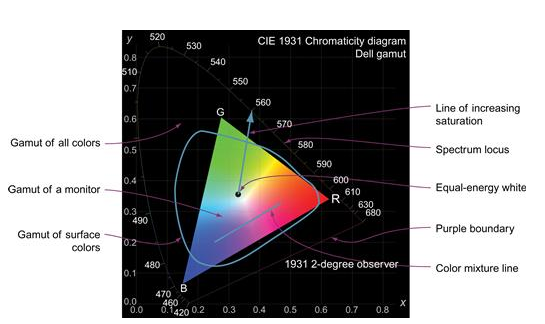
\includegraphics[width=0.4\textwidth]{cie_chromaticity.png}
        \caption{The CIE chromaticity diagram (interesting features)}
    \end{figure}


\end{multicols}\end{mdframed}


\begin{mdframed}\begin{multicols}{2}
\subsection{Opponent Process Theory}
\begin{compactdesc}
    \item[Opponent-pairs] Cornerstone of modern color theory.
        Black-white, yellow-blue and red-green lie on the same axis.
    \item[Naming] impossible: reddish green, yellowish blue. Confirmed.
    \item[Cross-cultural naming] 100 languages! Primary color terms are
        consistent, first are black and white. Next is red. The fourth and
        fifth are always yellow or green. The sixth is always blue. Seventh is
        brown followed by pink, purple, orange, and gray in no order.
    \item[Unique hues] we can identify yellow to 2nm. Green is either at 514nm
        or 525nm (for $\frac{1}{3}$ of population). Mostly independent of
        luminance level.
    \item[Neurophysiology] Cells in primary visual cortexes of monkeys have the
        properties predicted by opponent process theory.
    \item[Categorical colors] colors close to the ideal primaries are easy to
        remember. Colors that are not basic, like orange or lime  green are
        difficult to remember. Only eight colors and white were accurately named.
\end{compactdesc}
\end{multicols}\end{mdframed}


\begin{mdframed}\begin{multicols}{2}
\subsection{Properties of color channels}
\begin{figure}[H]
\centering
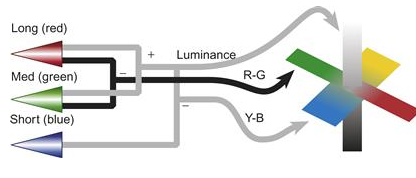
\includegraphics[width=0.4\textwidth]{opponents.png}
\caption{Opponent colors}
\end{figure}

\begin{figure}[H]
\centering
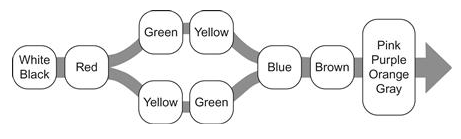
\includegraphics[width=0.4\textwidth]{color_order.png}
\caption{Cross cultural color order}
\end{figure}
\begin{figure}[H]
\centering
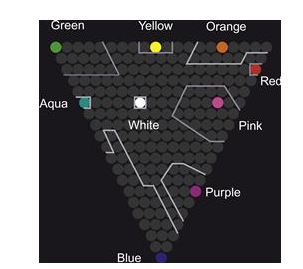
\includegraphics[width=0.6\linewidth]{accurately_identified.png}
\caption{8 colors identified 75\% of the time}
\end{figure}



\end{multicols}\end{mdframed}


\begin{mdframed}\begin{multicols}{2}
\subsection{Properties of color channels}
\begin{compactdesc}
    \item[Isoluminant/equiluminous] same grayscale. Stereo depth i
    \item[Spatial sensitivity] the two chromatic colors carry only one-third
         of the information that the grayscale does. Chromatic differences are
         not suited for displaying any kind of detail.
    \item[Stereoscopic depth] only detected using luminance.
    \item[Motion sensitivity] easier to see the motion of objects with
        different luminance, colored looks slower.
    \item[Form] we're very good at perceiving shapes; but if chromatic
        differences are used for textures, expect weaker looking surfaces.
    \item[Summary] red-green, yellow-blue inferior in most respects to
        luminance
\end{compactdesc}
\end{multicols}\end{mdframed}


\begin{mdframed}\begin{multicols}{2}
\subsection{Color appearance}
\begin{compactdesc}
    \item[Monitor surrounds] it is important to pay attention to the environment
        of a monitor, for it affects colors perceived.
    \item[Color constancy] we cannot see absolute colors, they depend entirely
        on surrounding colors. Tungsten light is much more yellower than
        sunlight, but this is not often noticed.
    \item[Color contrast] similar to lightness contrast (chapter 3), can
        distort readings of a color-coded map. Relative color is much more
        important than absolute color.
    \item[Saturation] high: far from the grayscale, low: dull or grayish.
        Few saturation steps can be accurately distinguished.
    \item[Brown] wtf. Dark yellow, but rarely referred to this way. People may
        need a reference white to see it. May not be distinguishable in a set
        of color codes.
\end{compactdesc}
\begin{figure}[H]
\centering
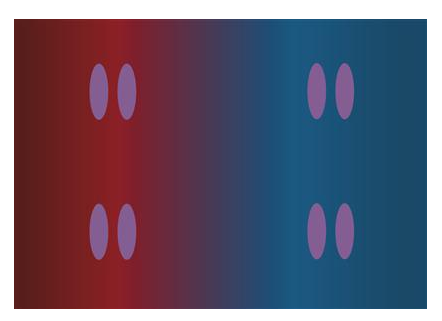
\includegraphics[width=0.4\linewidth]{color_contrast.png}
\caption{Color contrast illusion}
\end{figure}


\end{multicols}\end{mdframed}


\begin{mdframed}\begin{multicols}{2}
\subsection{App 1: Color specification interfaces}
\begin{compactdesc}
    \item[Color spaces] design a color picker! Best to offer a method showing
        colors on different backgrounds.
    \item[HSV] hue, value and saturation.
    \item[RGB] red, green and blue.
    \item[Color naming] People agree on few names. There exist large maps
        from intuitive names to actual values: NCS, Pantone (USA printing),
        Munsell (USA surfaces).
    \item[Color palettes] should provide ability to create personalized
        palettes.
\end{compactdesc}
\end{multicols}\end{mdframed}


\begin{mdframed}\begin{multicols}{2}
    \subsection{App 2: Color for labeling (nomial codes)}
    Perceptual factors to consider when picking a set of color labels.
\begin{compactdesc}
\item[Distinctness] uniform (equidistant) color space can be used to determine
    the difference between two colors. Must also consider background and area.
    \item[Unique hues] Red, green, yellow, blue, as well as black and white.
        Small set of color codes required.
    \item[Contrast with background] should consider different backgrounds.
        Always make sure there is a luminance difference if symbols must be
        distinguished from background.
    \item[Color blindness] Yellow-blue direction is most universal.
    \item[Number] Five to ten elements can fit in a color code.
    \item[Field size] Do not use very small color-coded areas. Yellow-blue is
        hard to distinguish at small sizes.
    \item[Conventions] Pay attention. Domain specific. Example: hot = red,
        cold = blue.
\end{compactdesc}
\begin{figure}[H]
\centering
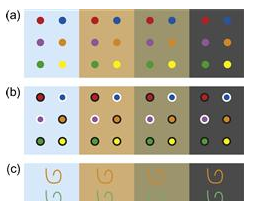
\includegraphics[width=0.4\textwidth]{colors_on_backgrounds.png}
\caption{Colors on different backgrounds. Lines especially difficult}
\end{figure}



\end{multicols}\end{mdframed}


\begin{mdframed}\begin{multicols}{2}
\subsection{App 3: Color sequences for data maps}
\begin{compactdesc}
    \item[Chloropleth map] representing continuous values on a map using color
    \item[Form and quantity] Different color sequences have different effects
        when used for ranking. Can be actively misleading. Best to use
        a straight line through a uniform color space. Could use a spiral
        sequence.
    \item[Interval pseudocolor sequences] contours and a discrete sequence
        of colors (not smooth) work well.
    \item[Ratio pseudocolors] if values are signed, such a sequence is called
        diverging or bipolar.
    \item[Sequences for the color blind] There are specially designed color
        sequences.
    \item[Bivariate color sequences] hue and lightness/saturation works well.
        Don't use color on two axes, they end up unreadable.
    \item[Best of the best] let a user with enough time decide what shows
        the most information for them.
\end{compactdesc}
\end{multicols}\end{mdframed}


\begin{mdframed}\begin{multicols}{2}
\subsection{App 4: Color reproduction}
    Most output devices cannot reproduce the 16 million colors that can be
    created by a monitor.


    Good mapping from one device to another:
\begin{compactenum}
    \item White should look white on both devices, same goes for black
    \item Maximum luminance contrast is desirable
    \item Few colors should lie outside target gamut
    \item Hue/saturation shifts should be minimized
    \item Increase in saturation is preferable to a decrease
\end{compactenum}
\begin{compactdesc}
    \item[Calibration] setup a common reference
    \item[Range scaling] scale about the luminance axis
    \item[Rotation] find the neutral white. The two white axes should coalign.
    \item[Saturation scaling] Scale radially.
    \item[Modern printers] use heuristics, though an educated technician can do
        better.
\end{compactdesc}
\end{multicols}\end{mdframed}



